\def\comment#1{{\hfil\scriptsize\color{gray}(* #1 *)}}
\def\tla{TLA$^+$}

\lecture{Lógica Temporal de Ações$^+$}{tlaplus}

\frame{\maketitle}

\begin{frame}{\tla}
  \begin{itemize}
  \item<1,4> \alert{\tla} é uma linguagem de especificação formal para especificar sistemas
    e algoritmos;
  \item<2,4> \href{https://lamport.azurewebsites.net/tla/tla.html}{\tla}~usa matemática simples para descrever os sistemas formalmente e é
    especialmente adequada para sistemas distribuídos e concorrentes;
  \item<3,4> A linguagem foi desenvolvida por
    \href{http://www.lamport.org/}{Leslie Lamport} a partir dos
    trabalho em Lógica Temporal de
    \href{https://cs.nyu.edu/faculty/pnueli/}{Amir Pnueli}.
  \end{itemize}
\end{frame}

\begin{frame}{\tla}{}
  Basicamente, iremos nos concentrar nos seguintes aspectos da linguagem:

  \begin{description}
  \item[Init]: Estado inicial da computação;
  \item[Invariant]: Propriedades que não variam durante a execução do sistema;
  \item[Next]: Próximo estado possível após o início da execução;
  \item[Spec]: Especificação do sistema.
  \end{description}
  
  
\end{frame}

\begin{frame}{Exemplos de Uso}\small
  \begin{itemize}[<+-| alert@+>]\setbeamercovered{transparent}
  \item Na Microsoft, um \textit{bug} crítico foi encontrado durante o
    processo de escrita da especificação em TLA$^+$ do modulo de
    memória no
    XBox.~[\href{http://channel9.msdn.com/Events/Build/2014/3-642\#time=21m46s}{ref}]
  \item Desde 2011, a Amazon usa TLA$^+$ para especificar alguns seus
    serviços críticos, tais como o Amazon Web
    Services~(AWS).~[\href{http://lamport.azurewebsites.net/tla/amazon.html}{ref}]
  \item TLA$^+$ tem sido usado para projetar o banco de dados Cosmos
    DB que faz parte da Microsoft Azurre. O Cosmos DB é um banco de
    dados globalmente distribuído com cinco modelos de
    consistência.~[\href{https://techcrunch.com/2017/05/10/with-cosmos-db-microsoft-wants-to-build-one-database-to-rule-them-all/}{ref1},
    \href{https://techcrunch.com/2017/05/10/with-cosmos-db-microsoft-wants-to-build-one-database-to-rule-them-all/}{ref2}]
  \end{itemize}
  
\end{frame}

\begin{frame}{Relógio alternado de 1-bit}{\em Alternate one-bit clock}
  VARIABLE $clk$  \comment{declaração da variável relógio}

  \pause

  \bigskip
   $Init$ == $clk = 0 \lor clk=1$ \comment{Inicialização}\\

  \pause
  \bigskip\begingroup

    \comment{Próximos estados}\hfill
    \begin{tabbing}
      $Next$ == \=$\lor$\= $\land clk = 0$\\
      \>\>$\land clk' = 1$\\
      \only<4->{
      \>$\lor$\= $\land clk = 1$\\
      \>\>$\land clk' = 0$
    }
    \end{tabbing}
  
\endgroup

\pause\bigskip

$Spec$ == $Init$ $\land$ [\ ][Next]$_{<<clk>>}$ \comment{Especificação}

\pause\medskip

{\scriptsize\color{blue} A especificação ($Spec$) é satisfeita ($true$) se o
  estado inicial ($Init$) é satisfeito ($true$) e cada passo satisfaz
  ($true$) [\ ][Next]$_{<<clk>>}$\footnote{\tiny [\ ] é o operador da lógica temporal
   chamado caixa ({\em box}).}}

\end{frame}

\begin{frame}[fragile]{Relógio alternado de 1-bit - impressão final}{\em Alternate one-bit clock}
  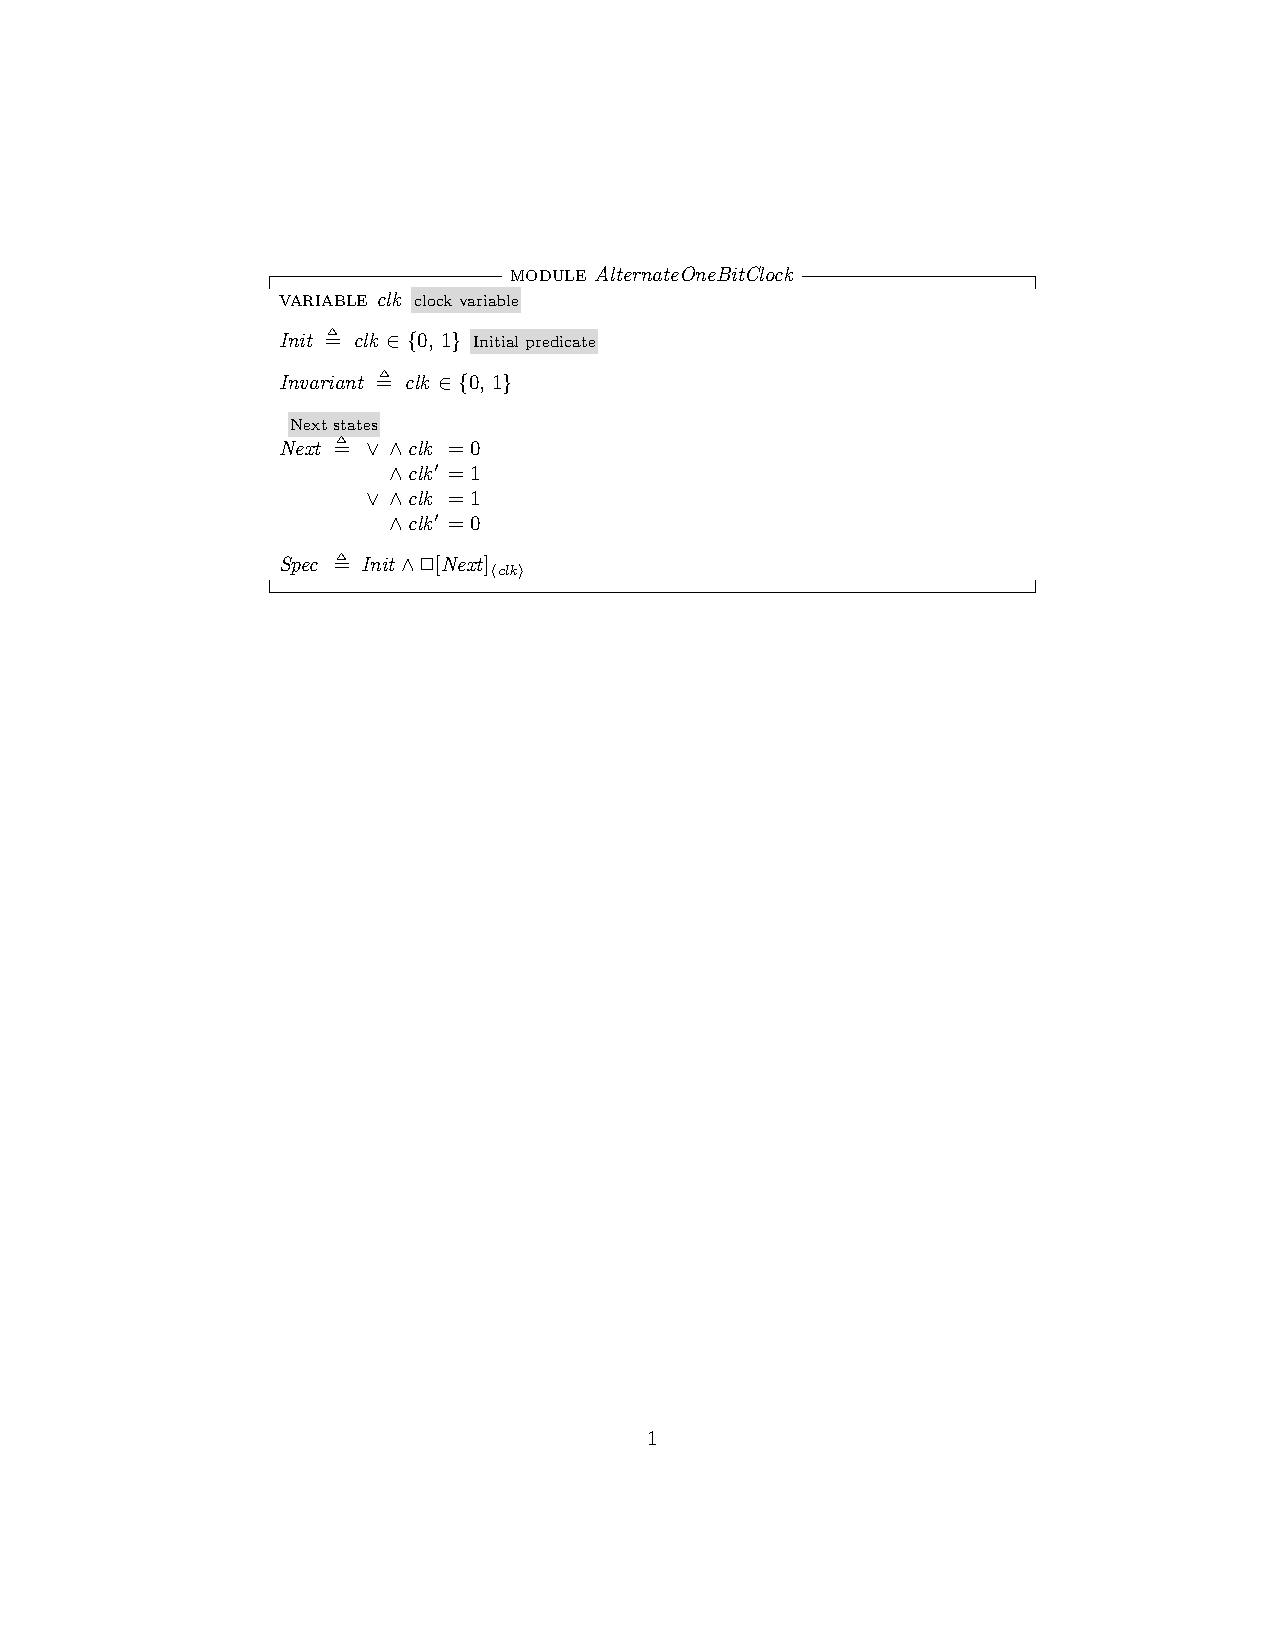
\includegraphics[scale=.6]{../src/AlternateOneBitClock.pdf}
\end{frame}

\input mdc

\begin{frame}{MDC}{Especificação completa}

  GCD - {\em Greatest Common Divisor}\\ {\tiny A expressão
    $PositiveInteger$ siginifica que qualquer número Natural pode ser
    escolhido desde que seja diferente de $0$. {\sc theorem} pode ser
    ignorado, por enquanto, para nosso propósito.}
  
  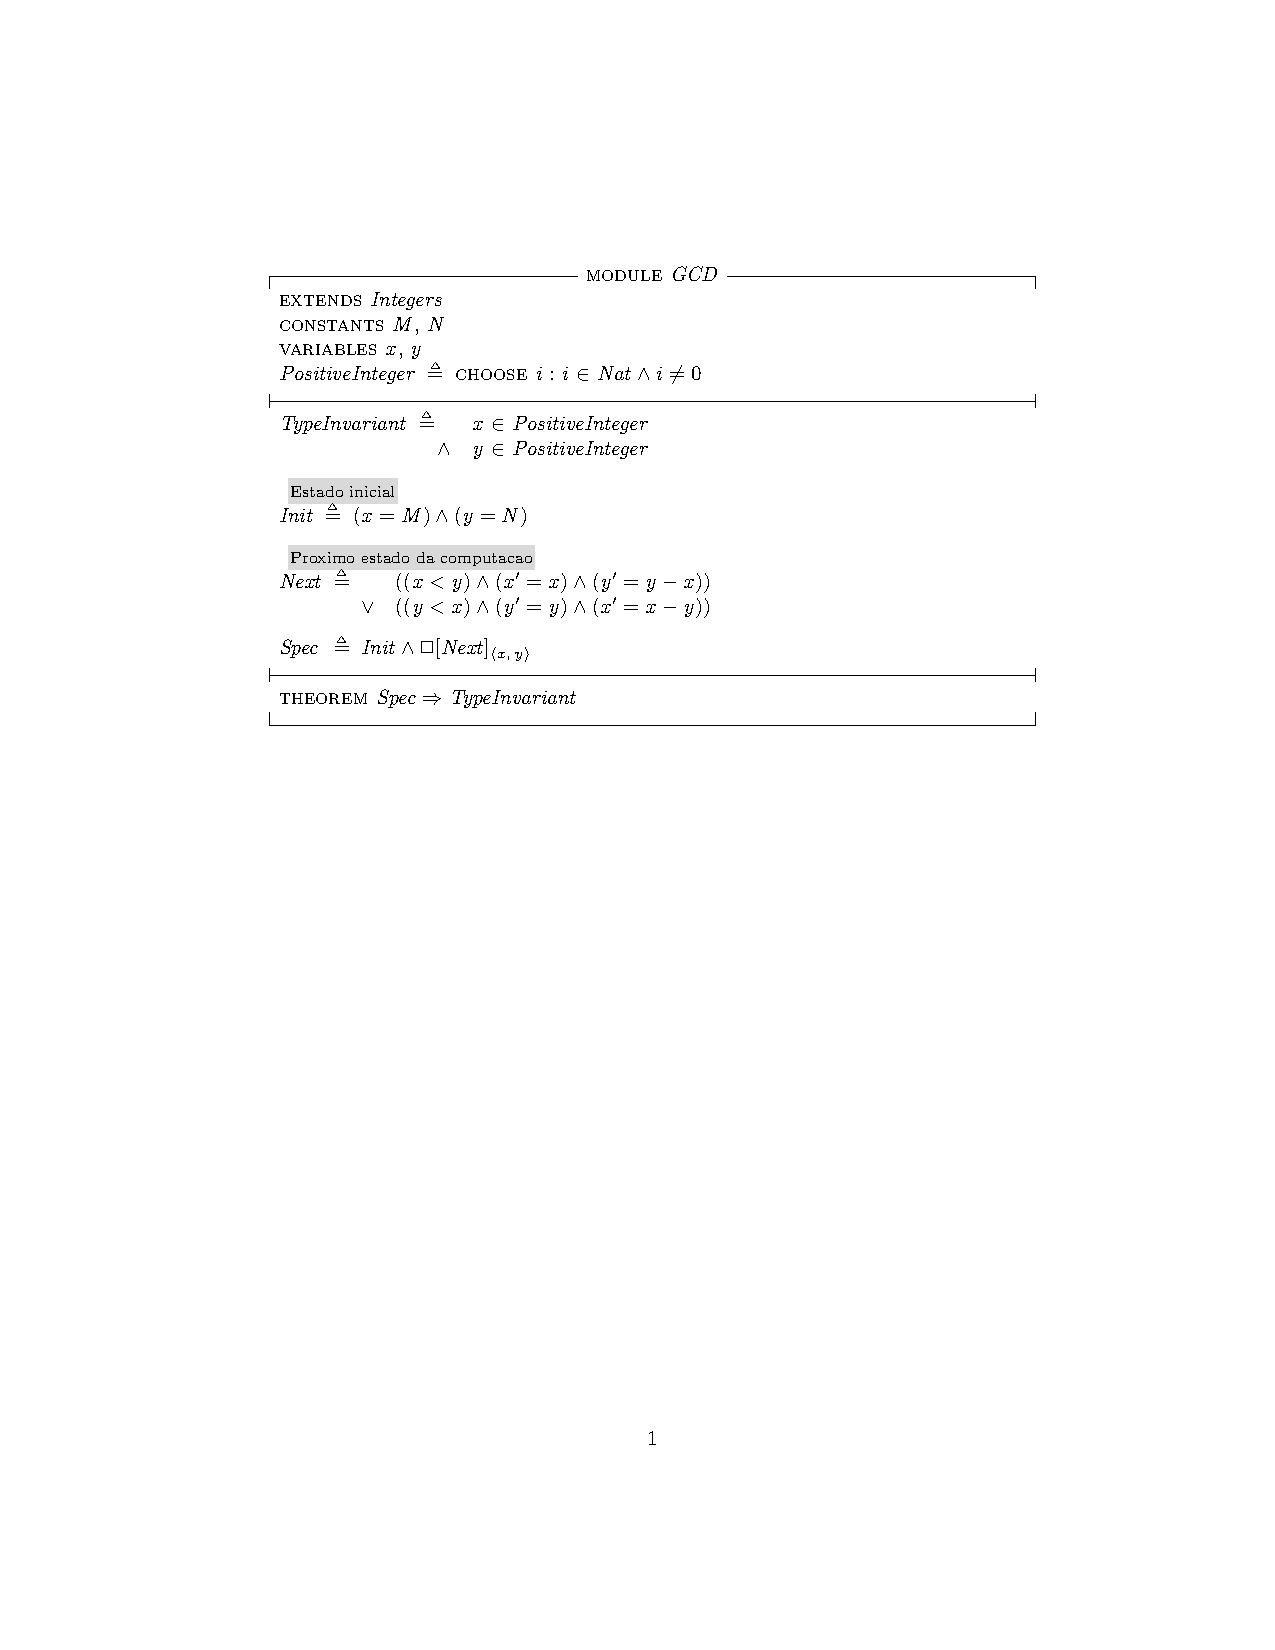
\includegraphics[scale=.5]{../src/GCD.pdf}
  
\end{frame}
